\chapter{評価実験}

\label{chap:evaluation}

\section{実験概要}
複数のタスクでネットワークを評価する。実験の目的を以下に示す
\\・4.2節では順序整理モジュールの有効性をablation studyにより検証する
\\・4.3節では提案する非分散型メモリの長期依存関係の計算能力を分散型の既存手法と比較する
\\・4.4節では提案ネットワークにおける関係推論能力を評価する
\\・4.5節ではより複雑な関係推論を必要とするタスクにおける性能をベースラインの関係推論ネットワークと比較する

全てのタスクにおいてネットワークはLSTMコントローラを採用し、ロジスティックシグモイド出力層を有する。
クロスエントロピーを損失関数として訓練し、最適化手法としてはAdamを用いた。
また、各入力系列の開始時にネットワークの隠れ状態はリセットされる。
各タスクにおけるネットワークのパラメータ、データのバッチサイズ、学習率を表Xに示す。

\subsection{priority sort}
priority sortタスクの入力・ターゲットの構成を図\ref{fig:priority}
入力系列はランダムなバイナリベクトルに、[-1,1]の範囲から一様分布に従い決定した乱数を優先度として付加したものからなる。
ターゲットは入力系列をこの優先度に従ってソートした系列の一部とする。
NTM中の設定に従い入力系列の長さは20ベクトル,ターゲットは系列の中から優先度が高い順に16ベクトルとする。

このタスクはネットワークが入力をソートする能力を評価する。

図\ref{fig:priority}
\begin{figure}[t]
	\centering
	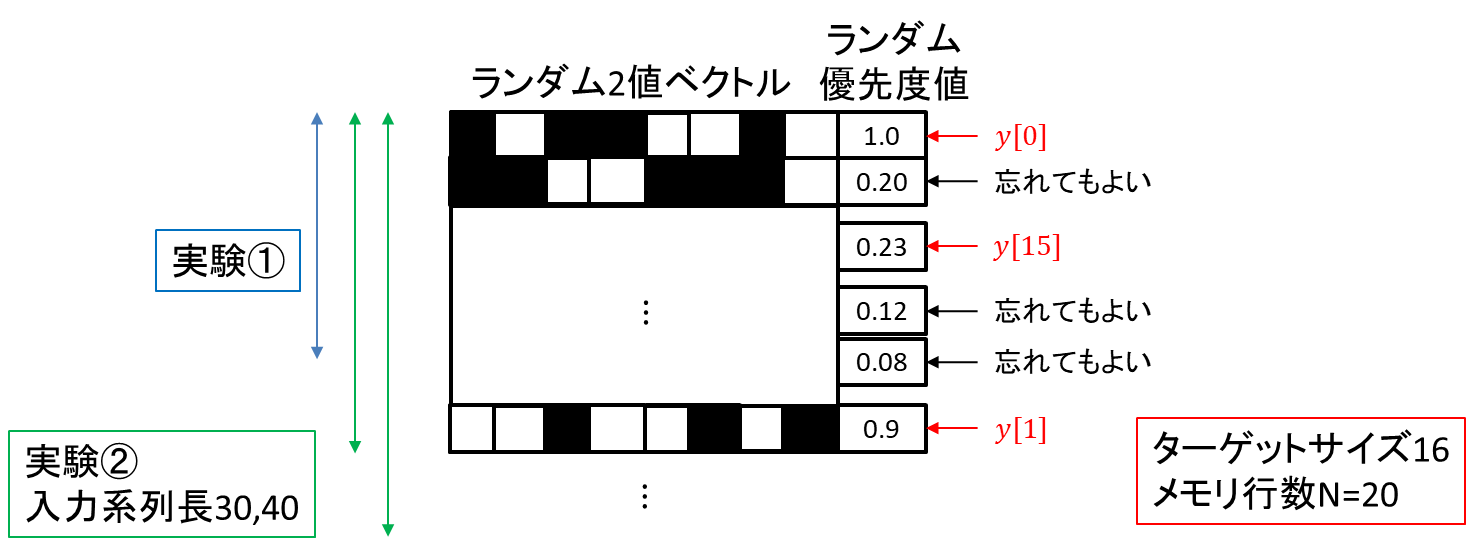
\includegraphics[width=\linewidth]{./figure/img_slide/priority.png}
	\caption{priority sort タスク}
	\label{fig:priority}
\end{figure}

\subsection{実験結果}
表\ref{table:result-1}に

\section{実験1 priority sortにおける長期入力系列の検証}
 4.2節のタスクにおいて入力系列のサイズを増加させたときの精度の推移を観察する。この実験により提案ネットワークが長期依存関係を扱う能力を評価する。
提案ネットワークは入力系列が長期にわたるとき、分散型項目メモリを持つSAMよりも正答率が高くなることが期待される。

\section{実験2 関係推論能力の評価}
\subsection{実験概要}
この実験の目的は提案手法がNTMに関係推論能力を付与出来るかを評価することである。
既存研究\cite{rrnn}\cite{sam}はRMCやSTMのような関係推論能力を持つモデルが90以上の精度を記録した一方で、NTMやDNCの精度は30を超えないことを示している。
提案ネットワークがNTMメモリ項目間の関係を計算できる場合、NTMよりも大きく改善された精度を示すことが期待される。

\subsection{タスク:Nth-farthest}
入力系列はランダムに生成されたバイナリベクトルからなる。ベクトルの次元を$d$、系列長を$l$で表したとき、タスクの要求は入力系列中のあるベクトル$m$から$n$番目に遠いベクトルを見つける事である。$m,n$は入力系列ごとにランダムに決定される。
1ステップあたりの入力はバイナリベクトル、ベクトルのID、$m$、$n$を連結したベクトルからなり、$ID,m,n∈\{1,2,…,l\}$はone-hotエンコーディングにより表現されるため、最終的な入力の次元は$d+3l$になる。
既存研究\cite{rrnn}に従い、$d=16,l=8$として実験を行った。

このタスクは入力の読み書きやソートといったタスクよりも複雑な処理をネットワークに要求する。
ネットワークは$m$と全入力のペアの距離を計算しソートを行う必要がある。距離は入力間の関係情報の一形態である。
入力そのものをソートするタスクと異なり、関係情報のソートの為に関係メモリを活用する必要がある。

\subsection{実験結果}
Nth-farthestタスクによりRMCおよび提案ネットワークを訓練したときの学習曲線を図\ref{fig:nth_result}に示す。
\begin{figure}[t]
	\centering
	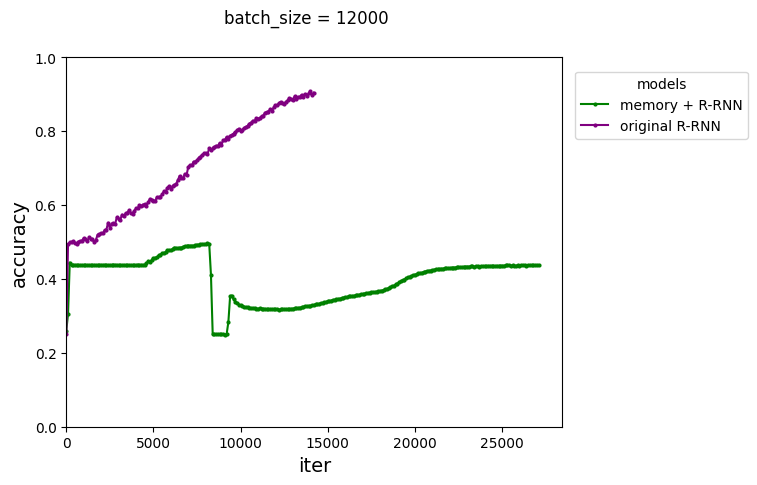
\includegraphics[width=\linewidth]{./figure/nth/orig_rrnn_id1.png}
	\caption{Nth-farthestタスクにおけるRMCおよび提案ネットワークの学習曲線}
	\label{fig:nth\result}
\end{figure}

\subsection{考察}
メモリそのまま入力 良くない 情報足りない
ヘッドで書き込みや読み書きに使った根拠 判断 しかし関係メモリは内容しか見ていない
NTMのヘッド内でメモリの更新や読み出しの判断に使用された情報は
これらを項目メモリに付与したい

SAMや\cite{working2mem}〜のような既存の2メモリモデルを見る限り、関係メモリから項目メモリの内容を復元する操作がある。今は項目→関係の一方向だけど逆も入れてメモリが相互作用できるようにする

samは項目メモリ内容の間の関係情報を関係メモリに保存する際に、線形変換で圧縮=項目の抽出?をしている。
入力が大きすぎて冗長なのが問題の場合、オートエンコーダのように圧縮・抽出したり、項目メモリ→関係メモリの部分のために読み出し操作をもう一つ実装するとよいかも

でかすぎたか RMCはもともと1ベクトルを入力 無理やり拡張した クエリとの齟齬も

\cite{working2mem}は
短期記憶として項目を保存するところに関係推論をかけている
時間で並んでいる
忘却機構により項目メモリを固定長に保てるという利点があるが
これと比較すると
ヘッドの情報無いんだから 関係メモリが見る順番バラバラでは
時間順序に関する情報を別に保存するか、時間とは別の基準をもってメモリの項目を一貫性を持った並びに

時間順序に着目すると DNCのlink matrix

\section{実験3 関係推論能力改善の検証}
\subsection{実験概要}
実験2の考察を踏まえ、項目メモリへの書き込みに関する情報を用いて関係メモリの入力を改善し、項目メモリと関係メモリの連携を強化することを試みた。
実験では4種類の異なる方法で変更を加えたモデルの性能をNTMや提案ネットワークと比較し,評価した。
1つ目のモデルでは式\ref{eq:w_sum}で計算される,書き込み重みの総和$q_t$に基づき項目メモリをソートしたものを関係メモリへの入力とした。
このモデルではヘッドにおける計算の内容を直接提示することではなく、関係メモリの入力を一貫性を持った並びにすることを目的としている。
入力系列全体を通して頻繁に提示される項目ほどコンテンツベースの重みによる更新が発生し、$q_t$は大きな値になると考えられる。
そのため関係メモリ内のself-attention入力層の重みは常に同程度の出現頻度の項目を提示されることが期待される。
ヘッドが複数存在する場合、全ヘッドの$q_t$の総和に基づいてソートを行う。
\begin{equation}\label{eq:w_sum}
	q_t=\sum_t{w^w_t}
\end{equation}
2つ目から4つ目のモデルでは書き込みに関する情報を項目メモリに新たな列として追加し,関係メモリへの入力とした。
ヘッドが複数存在する場合、ヘッドごとに異なる列として追加される。
2つ目では書き込み重みの総和$q_t$を追加した。
3つ目では式\ref{eq:w_sum_thr},\ref{eq:thr}に示すように、書き込み重みの各要素にしきい値処理を適用した値の総和$c_t$を追加した。
書き込み重みの総和を用いる試みでは、一つの行に一つの項目が強く書き込まれた場合と、弱い強度で数回書き込まれた場合の区別を付けることが出来ない。
3つ目の試みは0.1以上の強度の書き込みを全て一度の書き込みとみなし、各行の書き込み回数を保存・利用することを意図したものである。
\begin{equation}\label{eq:w_sum_thr}
	c_t=\sum_tf(w^w_t)
\end{equation}
\begin{equation}\label{eq:thr}
	f(w^w_t)(i)=
	\begin{cases}
	1 & (w^w_t(i) \geq 0.1)\\
	0 & (w^w_t(i) < 0.1)
	\end{cases}
\end{equation}
4つ目では最後に書き込みが行われた時間ステップの情報を項目メモリに追加した。
入力項目が提示された順序の情報を保持し、推論に利用することを目的としている。
付与される時刻は0-1に正規化され、書き込みが行われたかどうかの判定は3つ目の試みと同じく0.1をしきい値とした。

%4.1.1節及び4.1.2節ではネットワークの基礎的な記憶と項目整理の能力を評価する。
%NTM\cite{ntm}の評価で用いられたシンプルなアルゴリズムタスクを説明する。

\subsection{タスク:associative recall}
NTM\cite{ntm}の評価で用いられたシンプルなアルゴリズムタスクの一つである。
一定の長さのランダムに生成されたバイナリベクトルからなる系列を1アイテムとし、
始めにネットワークにはランダムな数のアイテムが入力される。
入力アイテム系列が提示された後、クエリとして入力アイテムのうちの一つが改めて入力される。
この時ターゲットとして、入力アイテムの中でクエリアイテムの次に提示されたアイテムを取る。
各アイテムの間および入力とクエリの間にはデリミタを表すベクトルが挿入される。
NTM\cite{ntm}中の設定に従い、ベクトルの次元を6,1アイテムの長さを3とし、アイテムの数は一様分布を用いて2-6のいずれかに決定する。

%以上の設定から入力系列の長さはデリミタを含め7-23,デリミタを除いた保存が必要な必要なベクトルに限ると6-18となる。既存研究\cite{ntm}ではメモリ行数は128に設定されており,これは全ての入力を順に保存するのに十分な。同じメモリ行に本実験では行数を12に設定した。

タスクはクエリアイテムをメモリから検索する、入力ベクトルを忠実に復元するといったメモリネットワークの基礎的な能力を要求する。
加えて、入力アイテムの順序の情報を保存する能力も要求する。

\subsection{実験結果}
Associative RecallタスクによりNTMおよび提案ネットワークを訓練した場合の学習曲線を図\ref{fig:ntm,rmc_m12id3}に示す。
\begin{figure}[t]
	\centering
	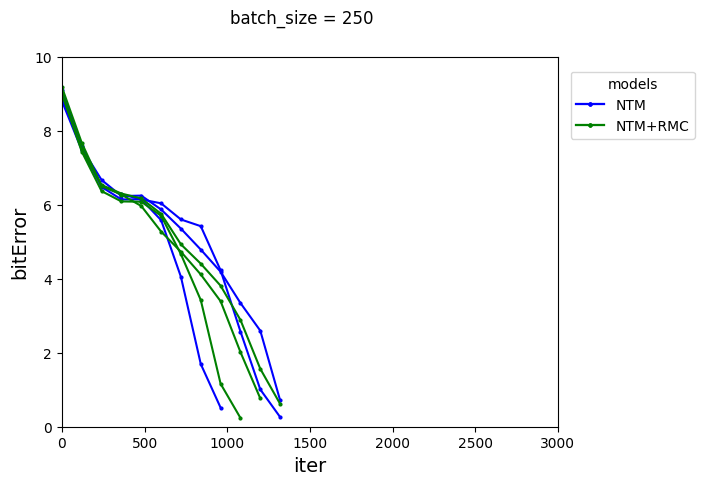
\includegraphics[width=\linewidth]{./figure/associative/ntm,rmc_m12id3.png}
	\caption{NTMおよび提案ネットワークの学習曲線}
	\label{fig:ntm,rmc_m12id3}
\end{figure}

書き込み重みの総和を付与した場合,および総和に従いソートを行った場合の学習曲線をNTMのものと共に図\ref{fig:ntm,sort,supple1}に示す。
各行の書き込み回数,最後に書き込んだ時刻を付与したモデルの学習曲線を図\ref{fig:ntm,supple2,3}に示す。
\begin{figure}[t]
	\centering
	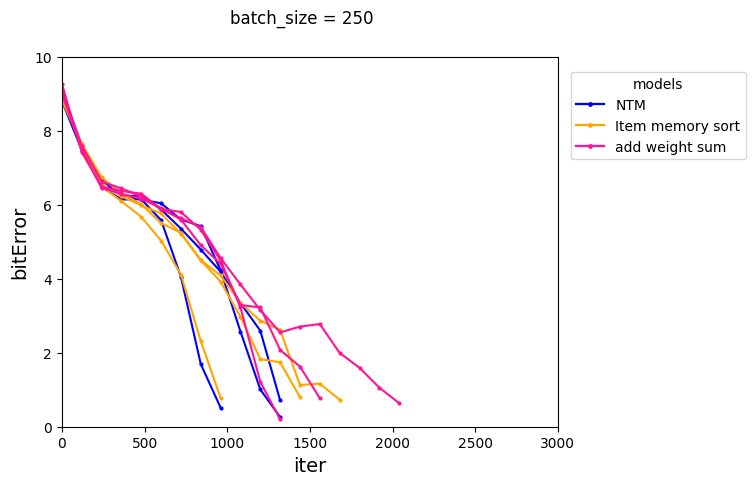
\includegraphics[width=\linewidth]{./figure/associative/ntm,sort,supple1_m12.png}
	\caption{NTMおよび提案ネットワークの学習曲線}
	\label{fig:ntm,sort,supple1}
\end{figure}
\begin{figure}[t]
	\centering
	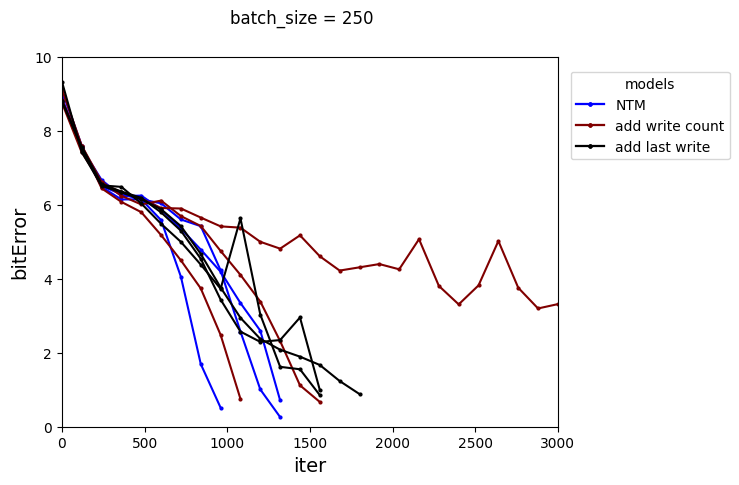
\includegraphics[width=\linewidth]{./figure/associative/ntm,supple2,3_m12.png}
	\caption{NTMおよび提案ネットワークの学習曲線}
	\label{fig:ntm,supple2,3}
\end{figure}

\subsection{考察}
結果からこのタスクにおいては、NTMと提案ネットワークの間に顕著な違いは確認されなかった。
重みの総和に基づくソートでも、平均して学習曲線に大きな変化はなかった。
重みの総和あるいは最後に書き込んだ時刻を付与した場合は,平均してエラー率の収束は遅くなったことが読み取れる。
書き込み回数を付与した場合,3回中2回の学習ではNTMに大きくは劣らなかったが1回では収束が大幅に遅れ,モデルの安定性に悪影響を与えたと考えられる。

唯一NTM・提案ネットワークから性能にほぼ悪化が無かったソートを適用したモデルでは、関係メモリの入力の列数に変化はなかった。
性能が悪化した3つのモデルでは関係メモリのサイズに変化はない一方で、各行への書き込みに関する情報として項目メモリに新たな列を付加していた。
これらを比較すると、付加した情報が余分な情報として他の情報が保存されるスペースを圧迫してしまったことが性能悪化の一因と考えられる。
改善として付加される列数=ヘッド数の分関係メモリのサイズを増加させることが考えられる。

最後に書き込んだ時刻および書き込み回数に改善が見られなかった一因として、しきい値処理が逆伝播不可な操作であることも考えられる。
メモリ操作をスキップしてヘッドの情報を関係メモリに渡すことを目的とした操作だが、スキップした接続を通して書き込み重みの計算を最適化可能にする点に改善の余地がある。
しきい値の代わりに急峻なsigmoid関数のような微分可能関数を適用した場合との比較も今後行いたい。

%項目メモリのソートが変化がないのが以外だった。
%self-attentionの変換の重みは位置により機能が分化すると思っていたので。改善か悪化すると思っていた

上の実験とは関係なく、実験2の考察を踏まえて、今後修士で試す予定の改善のこともいくつか考えていますがこれらは結論に書く形になると思います。ひとまず以下に箇条書きします
\\関係メモリをRMCではなくSAMにしてみる。もともとRMCは1メモリモデルで入力がベクトルなので、無理に拡張するよりこちらのほうがいいかも
\\SAMや\cite{working2mem}〜のような2メモリモデルを見る限り、関係メモリから項目メモリの内容を復元する操作がある。今は項目→関係の一方向だけど逆も入れてメモリが相互作用できるようにする
\\samは項目メモリ内容の間の関係情報を関係メモリに保存する際に、線形変換で圧縮=項目の抽出?をしている。
入力が大きすぎて冗長なのが問題の場合、オートエンコーダのように圧縮・抽出したり、項目メモリ→関係メモリの部分のために読み出し操作をもう一つ実装するとよいかも
\\似た話としてgraph attentionを利用して時間的・コサイン類似度的に近い項目に重み付けをしたセルフアテンションをかける。この結果を関係メモリに保存する(rmc,SAMとは異なる構造の関係メモリになる)

\begin{comment}
	また,ああああああ


\begin{table}[H]
	\caption{あああといいいの予測誤差}
	\centering
	\scalebox{0.98}[0.98]{
		\begin{tabular}{c|c|c|c|c|c|c}
			\multicolumn{1}{c}{} & \multicolumn{2}{|c|}{2019} 
			& \multicolumn{2}{c|}{2018} & \multicolumn{2}{c}{2017}\\ \hline \hline
			モデル    & ああ & いい & ああ & いい & ああ & いい \\ \hline
			Naive    & \bf{1} & 1 & \bf{1} & 1 & \bf{1} & 1 \\
			TCN      & 1.0895 & 0.9032 & 1.4791 & \bf{0.9198} & 1.2888 & 0.8555 \\
			LSTM     & 1.0384 & 0.9295 & 1.4917 & 0.9725 & 1.1627 & 0.8541 \\
			提案手法  & 1.0977 & \bf{0.8698} & 1.3824 & 0.9439 & 1.2061 & \bf{0.8516} \\
		\end{tabular}
	}
	\label{table:result-1}
\end{table}

\end{comment}